\documentclass[11pt, a4paper, spanish]{article}

\usepackage{alltt}

%%%%%%%%%% COMIENZO DEL PREAMBULO %%%%%%%%%%

%Info sobre este documento
\author{Mart\'n Cammi}
\title{Trabajo Pr\'actico de Algoritmos y Estucturas de datos III}

%\usepackage{infostyle}                                                  % provee un look & feel similar a un documento Word
\usepackage[top=2.5cm, bottom=2.5cm, left=2.5cm, right=2.5cm]{geometry}  % m\'argenes
\usepackage[ansinew]{inputenc}                                           % permite que los acentos del estilo \'a\'e\'i\'o\'u salgan joya
\usepackage[spanish, activeacute]{babel}                                 % idioma espaniol, acentos f\'aciles y deletreo de palabras
\usepackage{indentfirst}                                                 % permite indentar un parrafo a mano
\usepackage{caratula}                                                    % incluye caratula est\'andar
\usepackage{graphicx}                                                    % permite insertar gr\'aficos
\usepackage{color}                                                       % permite el uso de colores en el documento
\usepackage{amssymb}
\usepackage[pdfcreator={TexLive!, LaTeX2e con TeXnicCenter},
			pdfauthor={Grupo: "1"},
			pdftitle={Algoritmos III - Trabajo Pr\'actico 3},
			pdfsubject={Trabajo Pr\'actico 1},
			pdfkeywords={Prismas, Esferas, Punto de corte, puente, pizza},
			pdfstartview=FitH,            % Fits the width of the page to the window
			bookmarksnumbered,            % los bookmarks numerados se ven mejor...
			colorlinks,                   % links con bellos colores
			linkcolor=magenta]            % permite cambiar el color de los links
			{hyperref}                    % Permite jugar con algunas cosas que aparecer\'an en el PDF final

%RESTAURAR

\usepackage{algorithm}							% Permite tabular un codigo
\usepackage{algorithmic}
%\floatname{algorithm}{Algoritmo}
\renewcommand{\listalgorithmname}{Lista de algoritmos}
\renewcommand{\algorithmicrequire}{\textbf{Entrada:}}
\renewcommand{\algorithmicensure}{\textbf{Salida:}}
\renewcommand{\algorithmicend}{\textbf{fin}}
\renewcommand{\algorithmicif}{\textbf{si}}
\renewcommand{\algorithmicthen}{\textbf{entonces}}
\renewcommand{\algorithmicelse}{\textbf{si no}}
\renewcommand{\algorithmicelsif}{\algorithmicelse,\ \algorithmicif}
\renewcommand{\algorithmicendif}{\algorithmicend\ \algorithmicif}
\renewcommand{\algorithmicfor}{\textbf{para}}
\renewcommand{\algorithmicforall}{\textbf{para todo}}
\renewcommand{\algorithmicdo}{\textbf{hacer}}
\renewcommand{\algorithmicendfor}{\algorithmicend\ \algorithmicfor}
\renewcommand{\algorithmicwhile}{\textbf{mientras}}
\renewcommand{\algorithmicendwhile}{\algorithmicend\ \algorithmicwhile}
\renewcommand{\algorithmicloop}{\textbf{repetir}}
\renewcommand{\algorithmicendloop}{\algorithmicend\ \algorithmicloop}
\renewcommand{\algorithmicrepeat}{\textbf{repetir}}
\renewcommand{\algorithmicuntil}{\textbf{hasta que}}
\renewcommand{\algorithmicprint}{\textbf{imprimir}} 
\renewcommand{\algorithmicreturn}{\textbf{devolver}} 
\renewcommand{\algorithmictrue}{\textbf{cierto }} 
\renewcommand{\algorithmicfalse}{\textbf{falso }} 
 % mi archivo de traducci\'on			

%\selectlanguage{spanish}

%\selectlanguage{spanish}
\linespread{1.3}                    % interlineado equivalente al 1.5 l\'ineas de Word...
\pagestyle{myheadings}              %encabezado personalizable con \markboth{}{}
\markboth{}{Algoritmos III  - Trabajo Pr\'actico 3 - Cammi, Garbi, Kretschmayer}
\headsep = 30pt                     % separaci\'on entre encabezado y comienzo del p\'arrafo

%\addtolength{\oddsidemargin}{-2cm}	% configuracion IDEAL!!!
%\addtolength{\textwidth}{4cm}
%\addtolength{\textheight}{2cm}

% macro 'todo' para To-Do's
\def\todo#1{\textcolor{red}{#1}}

% Macro 'borde' para un texto con borde
\newsavebox{\fmbox}
\newenvironment{borde}[1]
{\begin{lrbox}{\fmbox}\begin{minipage}{#1}}
{\end{minipage}\end{lrbox}\fbox{\usebox{\fmbox}}\\[10pt]}

%%%%%%%%%% FIN DEL PREAMBULO %%%%%%%%%%

\begin{document}

\materia{Algoritmos y Estucturas de datos III}
\submateria{Segundo Cuatrimestre de 2011}
\titulo{Trabajo Pr\'actico 3}
\subtitulo{Cartero Chino en grafo mixto.}
\grupo{Grupo: `1'}
\integrante{Cammi, Mart\'in}{676/02}{martincammi@gmail.com}
\integrante{Garbi, Sebasti\'an}{179/05}{garbyseba@gmail.com}
\integrante{Kretschmayer, Daniel}{310/99}{daniak@gmail.com}

\maketitle

\thispagestyle{empty}

\tableofcontents

\newpage


\textbf{Ejecuci\'on del TP}
\label{sec:ejecucion}

	\subsection{Lenguaje utilizado}
		
		El lenguaje utilizado para el trabajo pr\'actico ha sido \emph{Java}, compilado con la versi\'on 1.5 de la Virtual Machine.
		
		El trabajo se acompa\~{n}a con los fuentes de la soluci\'on que puede importarse en IDE de Eclipse o ejecutarse desde l\'inea de comandos.

	\subsection{Como ejecutar el TP}
	
	\textbf{\underline{Desde l\'inea de comandos}}
	\begin{itemize}
			\item{Posicionarse en el directorio Algo3Tp3}
			\item{Copiar all\'i el archivo de entrada para el problema i, por ejemplo Ej.in}
			\item{Ejecutar el comando: \emph{java -cp ./bin problema1.Ej}}
	\end{itemize}
	Esto generar\'a el archivo Ej.out con la soluci\'on en el mismo directorio Algo3Tp3.

	\textbf{\underline{Desde el Eclipse}}
	
	Primero importaremos el proyecto:	
	
	\begin{itemize}
			\item{Seleccionar File $\Rightarrow$ Import.}
			\item{Seleccionar General $\Rightarrow$ Existing Projects into Workspace $\Rightarrow$ Next.}
			\item{Seleccionar el directorio llamado Algo3Tp3.}
			\item{Finish.}
	\end{itemize}
	
	Desde la vista de \textbf{Package Explorer} bajo el paquete \textbf{src} aparecer\'a el paquete \emph{algorithms} y dentro del el archivo de java:\\

	\begin{center}
		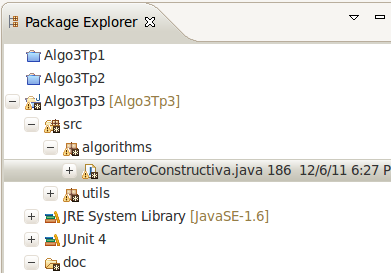
\includegraphics[scale=0.65]{others/packageExplorer.png}
	\end{center}

\newpage

	Para ejecutar un problema:

	\begin{itemize}
			\item{Posicionarse en el directorio Algo3Tp3}
			\item{Copiar en el directorio Algo3Tp3 el archivo de entrada para el problema i, por ejemplo Ej.in}
			\item{Con bot\'on derecho Run As $\Rightarrow$ Java Application. Se ejecutar\'a el problema seleccionado.}
	\end{itemize}
	Esto generar\'a el archivo Ej.out con la soluci\'on en el mismo directorio Algo3Tp3.

\newpage


\section{Introducci\'on}

	En 1736 Leonhard Euler public\'o un trabajo en el cual resolv\'ia el denominado \emph{problema de los puentes de K\"{o}nigsberg}. La ciudad de K\"{o}ningsberg, actual Kaliningrado, Rusia, est\'a dividida por el r\'io Pregel en 4 zonas, dos orillas, la isla de Kneiphof y otras dos partes divididas por el r\'io. Las orillas estaban conectadas mediante 7 puentes. El problema consist\'ia en partir de una orilla y recorrer todos los puentes, recorri\'endo una sola vez cada uno y volviendo al punto de partida.\\

Este fue el puntapi\'e inicial para un tipo de problema que m\'as adelante se modelar\'ia usando la teor\'ia de grafos. Este problema fue caracterizado por Euler y consist\'ia en encontrar un circuito que pasara por todas las aristas de un grafo una sola vez volviendo al punto de partida.\\
 
M\'as de doscientos a\~{n}os m\'as tarde en 1962 el matem\'atico chino Kwan Mei-Koo public\'o un paper en el que abordaba un problema ligeramente similar, donde propon\'ia que si un grafo no pose\'ia un circuito Euleriano, podr\'ia quiz\'as encontrar el circuito m\'as corto que pasara por todas las aristas aunque repitiera algunas de ellas. Este problema fue luego nombrado como "Problema del cartero chino".

\begin{center}
\centering 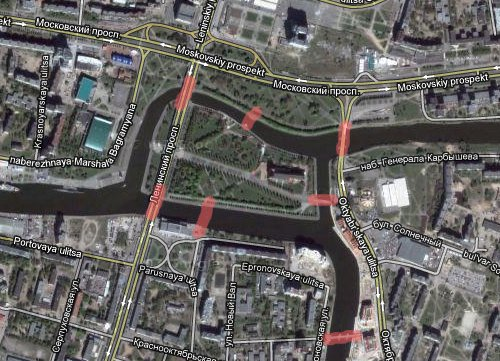
\includegraphics[scale=0.70]{img/KaliningradoBridges.jpg}\\
\small{Im\'agen actual de la ciudad de Kaliningrado, en rojo figuran los puentes del problema original de K\"{o}nigsberg, algunos de los cuales ya no existen hoy en d\'ia.}
\end{center}	

El problema tiene varias variantes, en este trabajo abordaremos la variante \emph{mixta} que consiste en intentar encontrar el m\'inimo circuito que pase por todas las aristas (no orientadas) y arcos (orientadas) de un grafo donde cada una tiene peso asignado.

\newpage
\section{Situaciones de la vida real}

    El algoritmo del cartero chino tiene m\'ultiples aplicaciones en la vida cotidiana, como por ejemplo:

	\begin{itemize}
	\item \emph{Camiones de basura}: en donde los camiones deban recorrer las calles de una ciudad y volver al centro de tratamiento de basura. Las calles estar\'ian representadas por aristas y las intersecciones por v\'ertices. Las calles podr\'ian bien tener diferentes sentidos o sentidos \'unicos, y los pesos podr\'ian corresponder a la cantidad de basura que deben recolectar en ciertas zonas (ej zonas industriales).
	\end{itemize}

	\begin{itemize}
	\item \emph{Reparto de Volantes:} C\'alculo de ruta \'optima que pase por todas las calles de una ciudad al menos una vez para poder repartir volantes de publicidad. Las calles estar\'ian representadas por aristas y las intersecciones por v\'ertices. Podr\'ia asignarse un peso de 1 a cada arista siendo que no tiene mayor complejidad repartir volantes en una u otra cuadra.
	\end{itemize}

\newpage
\section{Heur\'istica Constructiva}

	El \emph{algoritmo constructivo} se encargar\'a de tomar un grafo mixto y orientar sus aristas no orientadas y al mismo tiempo establecer un matching inicial.\\ Un matching consiste en agrupar pares de nodos ${(v,w)}$ tales que $d_{in}(v) > d_{out}(v)$ y\\ $d_{out}(w) > d_{in}(w)$.

\begin{center}
\centering 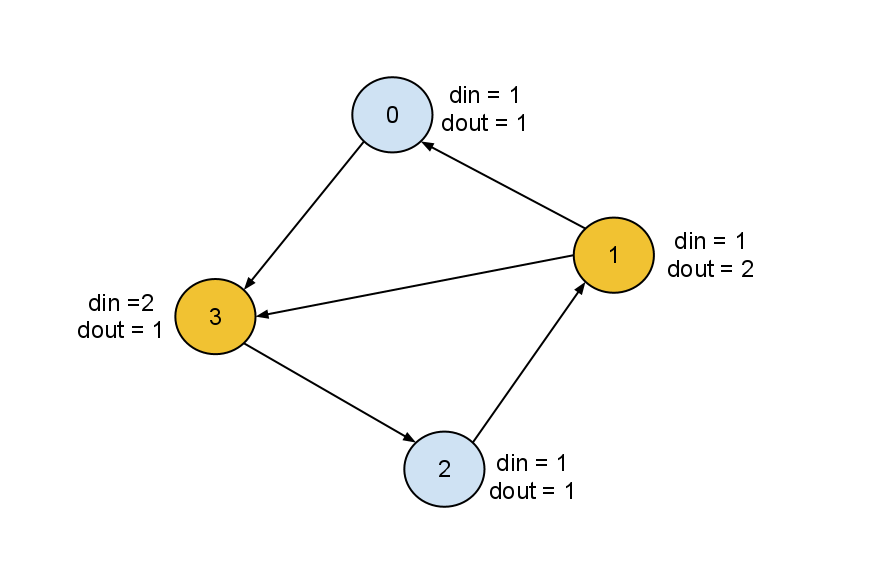
\includegraphics[scale=0.30]{img/Matching.png}\\
\small{En el grafo, los nodos 1 y 3 est\'an desbalanceados con respecto a $d_{in}$ y $d_{out}$, m\'as a\'un $d_{in} 3 > d_{out} 3$ y $d_{out} 1 > d_{in} 1$ con lo cual pueden formar parte de un matching: [(3,1)]}
\end{center}

\begin{center}
\centering 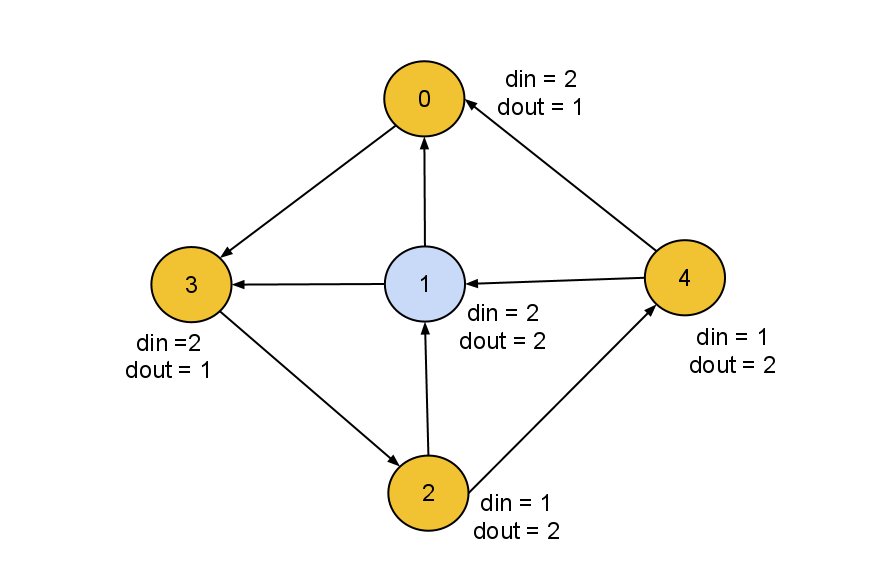
\includegraphics[scale=0.30]{img/Matching2.png}\\
\small{En el grafo, los nodos 0, 2, 3 y 4 est\'an desbalanceados con respecto a $d_{in}$ y $d_{out}$, un matching posible para equiparar sus $d_{in}$ y $d_{out}$ ser\'ia: [(0,2)(3,4)]}
\end{center}

	Para ello ideamos diferentes m\'etodos para la orientaci\'on de todas las aristas y fuimos experimentando con 5 m\'etodos distintos, todos ellos bas\'andose en los grados de los nodos para la elecci\'on de un nodo con el cual empezar a orientar sus aristas. Los m\'etodos elegir:\\
	
  \begin{itemize}
	\item 1) Los nodos que tienen igual cantidad de aristas sin orientar que orientadas, y que la suma de sus grados de entrada y salida sea mayor o igual a ALFA* nodoGradoMaximo.
	\item 2) Los nodos a partir de un cierto n\'umero, que viene como par\'ametro, y pondr\'a como m\'aximo ALFA* nodoGradoMaximo nodos.
	\item 3) Los nodos que tengan grado de nodo (sin orientar) mayor o igual al ALFA* nodoGradoMaximo.
	\item 4) Los nodos que tengan grado de entrada (orientado) mayor o igual al ALFA* nodoGradoMaximo.
	\item 5) Los nodos que tengan grado de salida (orientado) mayor o igual al ALFA* nodoGradoMaximo.
  \end{itemize}

Se entiende como \emph{nodoGradoMaximo} al nodo de mayor grado, contando aristas no orientadas.\\

Con cualquiera de estas posibilidades, siempre se intenta hacer un balance entre los grados que quedar\'an (solo quedar\'an grados de entrada y salida, ya que ser\'a completamente orientado). Realizando peque\~{n}as pruebas terminamos optando por el m\'etodo n\'umero 3) ya que por ejemplo con el m\'etodo n\'umero 1) no pod\'iamos asegurar que siempre existieran tales nodos que cumplieran la condici\'on.\\

El segundo m\'etodo se basa en encontrar los primeros ALFA * nodoGradoMaximo nodos, pero nos estaba dando nodos que pod\'ia tener grados menores que ALFA * nodoGradoMaximo, por lo que descartamos tambi\'en esta opci\'on.\\

En el cuarto y quinto m\'etodo se buscan los nodos que tengan $d_{in}$ o $d_{out}$ mayor o igual a la proporci\'on ALFA, pero esta proporci\'on estaba basada en el grado no orientado del nodo con mayor grado y est\'abamos comparando grados no orientados contra grados orientados que no ten\'ian necesariamente que tener relaci\'on.\\

Eligiendo el m\'etodo 3), podemos asegurarnos de siempre encontrar al menos un nodo ya que buscaremos aquellos que tengan grado mayor o igual a ALFA * nodoGradoMaximo donde el nodo de mayor grado estar\'a impl\'icitamente inclu\'ido ya que ALFA es un valor entre 0 y 1 que denota un porcentaje del nodoGradoMaximo.\\

Una vez que tenemos todo el grafo orientado, realizamos luego una etapa de matching entre los nodos que quedan con diferentes grado de entrada y de salida, y balanceamos a todos los nodos, para que queden con iguales grados de entrada como de salida, y el grafo quede Euleriano. Este matching lo calculamos con el peso del camino m\'inimo entre cada uno de los nodos, calculado sobre el grafo original utilizando Dantzig, ya que en esta etapa del algoritmo solo nos interesa saber el peso del camino m\'inimo y no como esta compuesto.\\


\newpage	
\section{Heur\'istica de b\'usqueda Local}

	El algoritmo de b\'usqueda local se encargar\'a, dado uno un grafo orientado completamente, un matching inicial y el grafo original, de buscar en la vecindad el mejor matching.\\

Un Matching est\'a compuesto por pares de la forma (nodoOrigen, nodoDestino).

Lo que haremos para conseguir una soluci\'on vecina es intercambiar en un matching los nodos destinos de dos pares para obtener as\'i un nuevo matching. Calculamos de esta manera todas las posibles soluciones vecinas intercambiando solo los nodos destinos de dos pares y luego de todas ellas obtenemos la que sea m\'inima y as\'i poder acercarnos a una soluci\'on mejor.\\

Esta definici\'on de vecindad tiene un tama\~{n}o de $\frac{k \cdot (k-1)}{2}$ donde $k$ es la cantidad de pares en el matching. Esto puede verse ya que para el intercambio de un par con otro existen $k-1$ posibilidades de otros pares. A su vez como la cantidad de pares en el matching est\'a determinada por la diferencia de grados de entrada y salida de los nodos, \'esta equivale a:\\


\begin{center}
	$\displaystyle{\frac{\displaystyle\sum_{i=1}^{n}{|d_{in}(i)-d_{out}(i)|}}{2}}$\\
\end{center}

\begin{center}
	$\displaystyle{\frac{\displaystyle\sum_{1 \leq i \leq n / d_{in} > d_{out}}^{}{d_{in}(i)-d_{out}(i)} + \displaystyle\sum_{1 \leq i \leq n / d_{out} > d_{in}}^{}{d_{out}(i)-d_{in}(i)} }{2}} \leq$\\
\end{center}

\begin{center}
	$\displaystyle{\frac{\displaystyle\sum_{1 \leq i \leq n / d_{in} > d_{out}}^{}{d_{in}(i)} + \displaystyle\sum_{1 \leq i \leq n / d_{out} > d_{in}}^{}{d_{out}(i)} }{2}} \leq $\\
\end{center}

\begin{center}
	$\displaystyle{\frac{m + m}{2} = \frac{2 \cdot m}{2} = m} $\\
\end{center}

As\'i, una vecindad tiene a lo sumo $m$ elementos.\\

A su vez la cantidad de posibles matchings diferentes que pueden existir es del orden de $k!$ ya en la elecci\'on de los nodoDestino para un nodoOrigen determinado existen $k$ posibilidades para su destino, una vez establecido para el siguiente nodo habr\'a $k-1$ posibles destinos y as\'i sucesivamente.

\newpage
Un ejemplo de una vecindad dado un matching inicial ser\'ia la siguiente:

\begin{center}
\centering 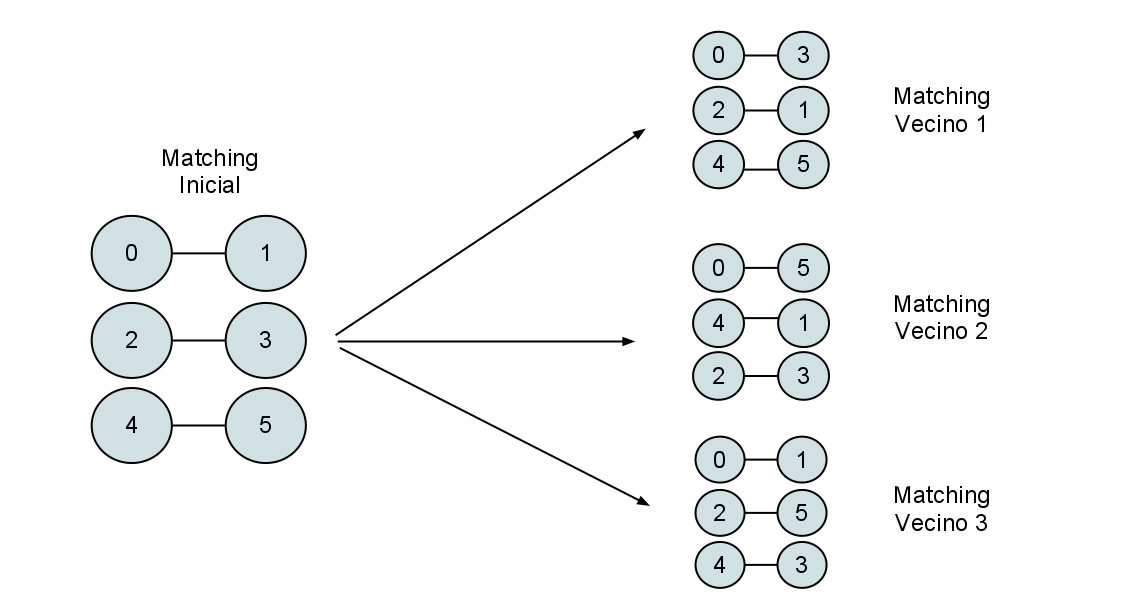
\includegraphics[scale=0.30]{img/MatchingVecindad.png}\\
\small{Una soluci\'on es vecina de otra si y solo si los matchings de ambas soluciones difieren s\'olo en un intercambio entre dos pares de matchings, as\'i, en el Vecino 1 se han intercambiado los pares (0,1) y (2,3) del matching original, en el Vecino 2 los pares (0,1) y (4,5) y en el Vecino 3 los pares (2,3) y (4,5).}
\end{center}

\newpage
\section{Metaheur\'istica Grasp}

Esta etapa del algoritmo realiza varias iteraciones de los algoritmos de las heur\'isticas constructiva y de b\'usqueda local, decidiendo mediante experimentaci\'on el nivel de aleatoriedad agregado al algoritmo constructivo, el tama\~{n}o de la vecindad a visitar y la cantidad de veces que se intentar\'a una soluci\'on nueva.\\
\noindent El parametro $ALFA$ es un valor perteneciente al intervalo $(0,1)$ y define el nivel de aleatoriedad del algoritmo constructivo.\\

\noindent El parametro $CANT\_ITERACIONES\_MAXIMA$ define el m\'aximo de veces que se construir\'a una soluci\'on inicial.\\

\noindent El parametro $CANT\_ITERACIONES\_SIN\_MEJORAR$ se usa como condici\'on de corte, si no se pudo encontrar una soluci\'on mejor en cierta cantidad de iteraciones de $GRASP$ se corta la ejecuci\'on y se devuelve la mejor hasta el momento.\\

\noindent El parametro $CANT\_ITERACIONES\_BUSQUEDA\_LOCAL$ define el tama\~{n}o m\'aximo que tendr\'a la vecindad ya que este puede ser exponencial en el tama\~{n}o del matching.\\


Como no tenemos el valor real de la soluci\'on \'optima, medimos la calidad de las soluciones como el porcentaje de peso agregado por el algoritmo en la soluci\'on con respecto al peso total de las aristas del grafo original. $\left(\frac{PesoCircuito - PesoAristas(G)}{PesoAristas(G)}\right)*100$\\
Las instancias utilizadas para tomar las mediciones fueron grafos de 100 a 500 nodos generadas pseudo-aleatoriamente.\\

\newpage
\subsection{Gr\'aficos de variaci\'on de ALFA}

\begin{center}
\centering 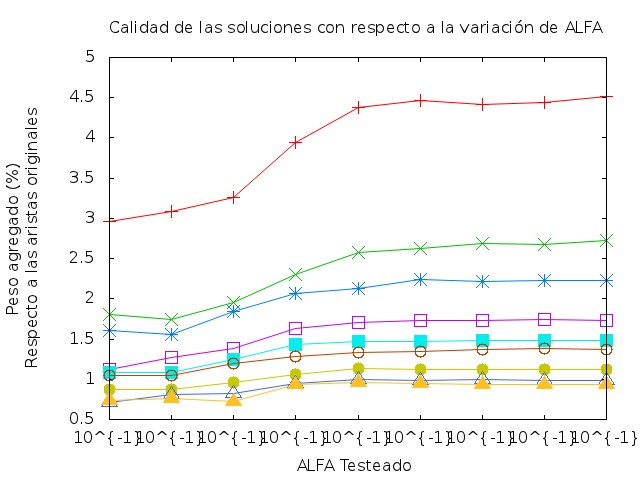
\includegraphics[scale=0.40]{img/VariacionAlfa.jpg}\\
\small{Este gr\'afico muestra la calidad de las soluciones con respecto a los valores para $ALFA$ testeados.}
\centering 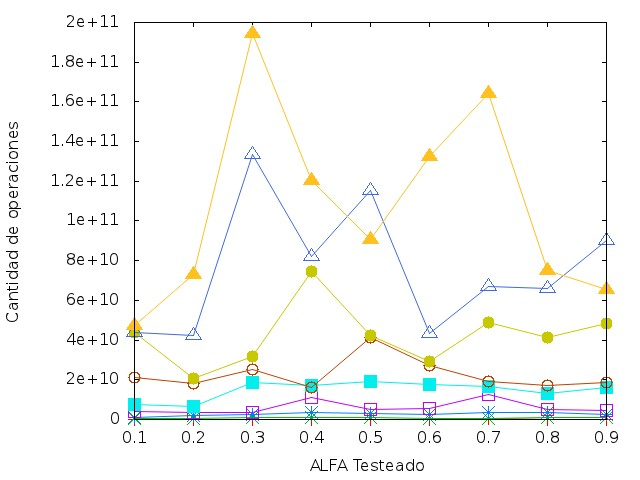
\includegraphics[scale=0.40]{img/VariacionAlfaComplejidad.jpg}\\
\small{Este gr\'afico muestra la cantidad de operaciones realizadas para los los valores de $ALFA$ testeados.}
\end{center}
Como se puede observar en los gr\'aficos de las mediciones tomadas para las mismas instancias con distintos valores para $ALFA$, se obtuvieron los mejores resultados para el valor $0,1$ y las complejidades pr\'acticas para ese valor son bastante razonables. El valor decidido para $ALFA$ fue entonces de $0,1$.\\

\newpage
\subsection{Gr\'aficos de cantidad de iteraciones}

\begin{center}
\centering 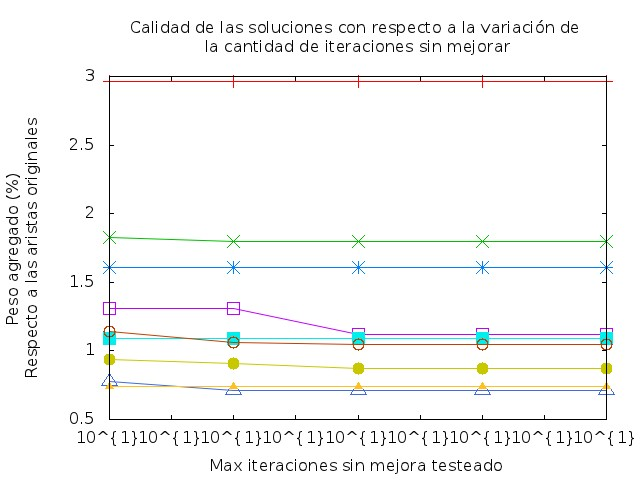
\includegraphics[scale=0.40]{img/VariacionItSinMejora.jpg}\\
\small{El gr\'afico muestra la calidad de las soluciones con respecto a los los valores para $CANT\_ITERACIONES\_SIN\_MEJORAR$ testeados}\\
\end{center}
\begin{center}
\centering 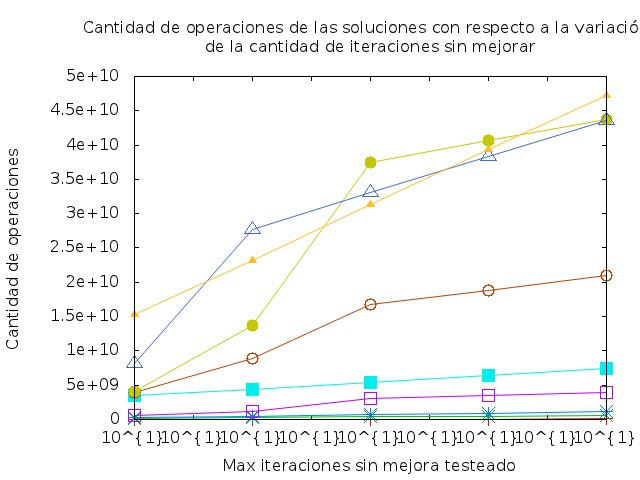
\includegraphics[scale=0.40]{img/VariacionItSinMejoraComplejidad.jpg}\\
\small{Este gr\'afico muestra la cantidad de operaciones realizadas para los los valores de $CANT\_ITERACIONES\_SIN\_MEJORAR$ testeados.}\\
\end{center}
Decidimos darle el valor $10$ a $CANT\_ITERACIONES\_SIN\_MEJORAR$ ya que en las mediciones tomadas se observa un incremento considerable en la cantidad de operaciones, mientras que las soluciones no mejoran de manera significativa.\\

El valor decidido para $CANT\_ITERACIONES\_MAXIMA$ fue $200$, ya que en ninguno de los casos evaluados lleg\'o a cortar por esa cota.\\
%El valor decidido para $CANT\_ITERACIONES\_BUSQUEDA\_LOCAL$ fue $50$.\\
\newpage
\section{Pseudo-algoritmo}

El siguiente es un pseudo-c\'odigo del algoritmo heur\'istico que realizamos para obtener el circuito Euleriano:\\

\noindent{\textbf{Algoritmo GRASP}}\\
Mientras no se superen las $I$ iteraciones totales y las $J$ iteraciones sin mejorar de $GRASP$ hacer:

\begin{itemize}
	\item \textbf{Algoritmo Constructivo}
		\begin{itemize}
			\item 1) Calular Dantzig sobre el grafo.
			\item 2) Orientar todas las aristas no orientadas del grafo.
			\item 3) Obtener un matching inicial entre los nodos que tengan $d_{in}$ $\neq$ $d_{out}$.
		\end{itemize}
	\textbf{Fin Algoritmo Constructivo}

	\item \textbf{Algoritmo B\'usqueda Local}\\
	\emph{Mientras} no se superen $K$ iteraciones y no se haya encontrado un matching \'optimo hacer
	\begin{itemize}
		\item 4) Obtener los matchings vecinos y quedarse con el m\'inimo vecino
	\end{itemize}
	\emph{Fin Mientras}\\
	\textbf{Fin Algoritmo B\'usqueda Local}

	\item 5) Calcular los caminos m\'inimos entre los nodos del matching.
	\item 6) Calcular el circuito Euleriano\\


\end{itemize}


\newpage

\section{Complejidad}
Complejidades donde $n$ es la cantidad de nodos, $m_{1}$ la cantidad de aristas, $m_{2}$ la cantidad de arcos y $m$ = $m_{1} + m_{2}$ \\
\begin{itemize}
	\item Inicializar grafo (lectura de archivo)
	\begin{itemize}
		\item Inicializar la matriz de pesos $O(n^{2})$
		\item Inicializar las listas de adyacencias $O(n + m_{1} +m_{2})$
	\end{itemize}
	En total: $O(n^{2} + m_{1} +m_{2}) \subseteq O(n^{2})$
	\item FuertementeConexo
	\begin{itemize}
		\item Inicializaci\'on de listas de adyacencias $O(n + m_{1} + m_{2})$
		\item resetVisitados y checkVisitados recorren un array de bools de tama\~{n}o $n$. $O(n)$
		\item visitarNodos recorre recursivamente en DFS las adyacencias y marca los nodos que son accesibles desde el nodo $0$. $O(m_{1} + m_{2})$
	\end{itemize}
	En total: $O(n + m_{1} + m_{2})$
	\item Calcular Dantzig
	\begin{itemize}	
		\item Inicializaci\'on de la matriz de pesos de caminos m\'inimos $O(n^{2})$
		\item 3 for anidados de $0$ a $n$ con operaciones de tiempo constante $O(n^{3})$
	\end{itemize}
	En total: $O(n^{3})$
	\item sumaPesosEjes recorre todas las aristas y arcos de los nodos $O(m_{1} + m_{2})$
	\item Clonar el grafo $O(n^{2} + m_{1} + m_{2})$ para copiar las estructuras
	\item orientarTodasAristas
	\begin{itemize}
		\item $m_{1}$ iteraciones de
		\begin{itemize}
			\item encontrarNodoAOrientar: Busca cuales nodos cumplen la condici\'on dada $O(n)$
			\item eleccionNodoAOrientar: Elije segun el parametro pasado por cual nodo de la lista anterior va a continuar $O(n)$
			\item orientarNodo $O(1)$
		\end{itemize}
		$O(1+ n+ n) \subseteq O(n)$
	\end{itemize}
	En total: $O(m_{1} * n)$
\newpage
	\item encontrarMatchingNodos
	\begin{itemize}
		\item Inicializaci\'on de arreglos de longitud $n$ $O(n)$
		\item para cada exedente de $D_{in}$ arma una pareja con un $D_{out}$ y lo agrega en una lista con el peso calculado con $Dantzig$ $O(\frac{\sum_{i=1}^{n}{|d_{in}(i)-d_{out}(i)|}}{2})$ $\subseteq$ $O(m)$
	\end{itemize}
	En total: $O(m + n)$
	\item encontrarMatchingDeMenorPeso: Dado un matching de tama\~{n}o $k$ devuelve el mejor matching que se puede obtener intercambiando los destinos de solo dos items del matching original. \\En total: $O(k^{2})$
	\item pesoMatching recorre una lista de tama\~{n}o a lo sumo $m$\\
	En total: $O(m)$
	\item agregarCaminosMatcheados
	\begin{itemize}
		\item Inicializaci\'on de matriz de tama\~{n}o $n*n$. $O(n^{2})$
		\item Para cada eje $(i,j)$ del matching (a lo sumo $m$ ejes)
		\begin{itemize}
			\item Si no esta calculado el $Dijkstra$ para el nodo $i$ $\rightarrow$ Calcula $Dijkstra$ sobre el grafo original y lo guarda. $O(n^{2})$
			\item Recuperar el camino del $Dijkstra$ calculado para el nodo $i$ hasta el nodo $j$. $O(n)$
		\end{itemize}
		$O(n^{2})$ Si no esta calculado $Dijkstra$ (a lo sumo $n$ casos)\\
		$O(n)$ Si ya esta calculado $Dijkstra$
	\end{itemize}
	En total: $O(m*n + n*n^{2})$ como $O(m)$ $\subseteq$ $O(n^{2})$ $\Rightarrow$ $O(m*n + n^{3})$ $\subseteq$ $O(n^{3})$
	\item Dijkstra
	\begin{itemize}
		\item Inicializaci\'on de arreglos de int y bool de tama\~{n}o $n$. $O(n)$
		\item Para cada nodo $i$ ($n$ elementos)
		\begin{itemize}
			\item Minvertex $O(n)$
			\item Para cada adyacente del nodo $i$ actualiza el valor $O(d(i))$
		\end{itemize}
	\end{itemize}
	En total: $O(n + \sum_{i=1}^{n}{(d(i) + n)})$ $\subseteq$ $O(n + 2*m + n*n)$ $\subseteq$ $O(n^{2})$
	\item encontrar circuito euleriano $O(2 *$ largo del circuito$)$\\
	Donde largo del circuito puede ser en peor caso $m*n$ cuando todos los nodos tiene matching y todos los caminos agregados tiene longitud $n$.\\
	En total: $O(m*n)$
\end{itemize}
\newpage

\begin{algorithm}
	\caption{Main($grafo$)}
	\begin{algorithmic}
	\STATE Grafo $GrafoOriginal$ $\gets$ Inicializar con instancia
	\IF{ es fuertemente Conexo $GrafoOriginal$}
		\STATE $PesosCaminosMinimos$ $\gets$ calcularDantzig($GrafoOriginal$)
		\STATE $SumaOriginalPesos$ $\gets$ sumaPesosEjes($GrafoOriginal$)
		\STATE $SumaSolucionMejor$ $\gets$ $\infty$, $MatchingMejor$ $\gets$ $\emptyset$
		\STATE $GrafoCopiaMejor$ $\gets$ $NULL$
		\WHILE{ no se alcanzan $MaximoIteracionesGrasp$ $\land$ $MaximoIteracionesSinMejoraGrasp$}
			\STATE Grafo $GC$ $\gets$ copiarGrafo($GrafoOriginal$)
			\STATE $ParametroGRASP$ $\gets$ Random
			\STATE orientarTodasAristas($GC$,$ParametroGRASP$)
			\STATE $matching$ $\gets$ encontrarMatchingNodos($GC$,$ParametroGRASP$)
			\WHILE{ no se alcanza $MaximoIteracionesBusquedaLocal$ $\land$ no se encontr\'o un matching \'optimo}
				\STATE $matching$ $\gets$ encontrarMatchingDeMenorPeso($matching$, $pesosCaminosMinimos$)
			\ENDWHILE
			\STATE $pesoMatching$ $\gets$ pesoMatching($matching$)
			\STATE $sumaSolucion$ $\gets$ $pesoMatching + SumaOriginalPesos$
			\IF{ mejor\'o la soluci\'on }
				\STATE $SumaSolucionMejor$ $\gets$ $sumaSolucion$
				\STATE $GrafoCopiaMejor$ $\gets$ $GC$
				\STATE $MatchingMejor$ $\gets$ $matching$
			\ENDIF
		\ENDWHILE
		\STATE agregarCaminosMatcheados($GrafoCopiaMejor$, $MatchingMejor$, $GrafoOriginal$)
		\STATE $circuito$ $\gets$ encontrarCircuitoEuleriano($GrafoCopiaMejor$)
		\RETURN $circuito$
	\ELSE
		\RETURN No hay Tour porque el grafo no era fuertemente conexo
	\ENDIF
	\end{algorithmic}
\end{algorithm}

\newpage

Complejidad:
	\begin{itemize}
	\item $O(n^{2})$ de inicializaci\'on
	\item $O(n + m_{1} + m_{2})$ de fuertementeConexo
	\item $O(n^{3})$ de Dantzig
	\item $O(m_{1} + m_{2})$ de sumarPesosEjes
	\item $MaximoIteracionesGrasp$ $*$
	\begin{itemize}
		\item $O(n^{2} + m_{1} + m_{2})$ de copiar el grafo
		\item $O(m_{1} * n)$ de orientarTodasLasAristas
		\item $O(m_{1} + m_{2} + n)$ de encontrarMatchingNodos
		\item $MaximoIteracionesBusquedaLocal$ $*$
		\begin{itemize}
			\item $O(m^{2})$ de encontrarMatchingDeMenorPeso
		\end{itemize}
		\item $O(m)$ de calcular peso del matching
	\end{itemize}
	\item $O(n^{3})$ de agregarCaminosMatcheados
	\item $O(m*n)$ de encontrar el CircuitoEuleriano
	\end{itemize} 
Para grafos que no son fuertemente conexos la complejidad es $O(n^{2} + m)$\\
Para las instancias interesantes del problema la complejidad esta dada por:\\
$O(n^{2} + n + m + n^{3} + m + \\MaximoIteracionesGrasp*(n^{2} + m + m_{1} * n + m + n + MaximoIteracionesBusquedaLocal*(m^{2}) + m ) + n^{3} + m*n)$ $\subseteq$
$O(n^{3} + m^{2} + m*n)$ $\subseteq$ $O(n^{3} + m^{2})$\\
%Como sabemos que el grafo es fuertemente conexo $\Rightarrow$ $ O(n) \subseteq O(m)$ $\Rightarrow$ la complejidad es\\
%$O(n^{3} + m^{2})$ $\subseteq$ $O(n*m^{2})$
\\
Definimos el tama\~{n}o de entrada como:

	\begin{center}	
	$T = log(n) + log(m_{1}) + log(m_{2}) + \displaystyle\sum_{i=1}^{m_{1} + m_{2}}{(log(eje_{i_{nodo1}})+log(eje_{i_{nodo2}}) + log(eje_{i_{peso}}))}$\\
	\end{center}

	\noindent Como $log(n) + log(m_{1}) + log(m_{2}) > 0 \Rightarrow$
	\begin{center}
	$T > \displaystyle\sum_{i=1}^{m_{1} + m_{2}}{(log(eje_{i_{nodo1}})+log(eje_{i_{nodo2}}) + log(eje_{i_{peso}}))}$\\
	\end{center}

	\noindent Tambi\'en sabemos que para cada eje $log(eje_{i_{nodo1}})+log(eje_{i_{nodo2}}) + log(eje_{i_{peso}}) > 1$ porque se necesitan al menos un bit para representar a cada eje $\Rightarrow$\\
	\begin{center}
	$T > \displaystyle\sum_{i=1}^{m_{1} + m_{2}}{1} = m_{1} + m_{2} = m$ \\
	\end{center}
	Sabemos que el grafo es fuertemente conexo as\'i que $n$ es del orden de $m$ $\Rightarrow$

	\begin{center}
	$T > m \geq n$ \\
	Dado la complejidad calculada y las cotas para $T$ vale $O(n^{3} + m^{2})$ $\subseteq$ $O(T^{3}+T^{2})$ $\subseteq$ $O(T^{3})$
	\end{center}
\newpage


\section{Conclusiones}

	Es interesante trabajar con problemas para los cuales un algoritmo exacto no sea una opci\'on en materia de tiempo. En el dise\~{n}o de este algoritmo heur\'istico nos dimos cuenta que el an\'alisis de los par\'ametros y que valores asignarle no es sencillo. Realizando las mediciones nos encontramos con grafos que con ciertos valores de los par\'ametros se encontraban mejores soluciones que otros, pero a su vez, estos mismos valores no mejoraban considerablemente las soluciones de otros grafos.\\

No solo eso, el algoritmo deb\'ia terminar en un tiempo considerable, y un aumento en la complejidad pod\'ia hacer decidirnos por sacrificar una soluci\'on levemente mejor por obtener un algorimo m\'as r\'apido. As\'i por ejemplo terminamos decidiendo para el par\'ametro ALFA que nos determinaba la amplitud de la vecindad un valor relativamente bajo justificaba ya la calidad de las soluciones que obten\'iamos opuestamente a utilizar un ALFA algo mayor que, mejorando la soluci\'on levemente, aumentaba la complejidad de manera considerable.\\

Es por eso que los algoritmos heur\'isticos se construyen a base de prueba y error, sin descartar claro est\'a una base te\'orica, para determinar que valores de los par\'ametros son los m\'as adecuados para tratar, en el caso de los grafos, la mayor generalidad posible. 


\end{document}
